\documentclass[letterpaper,11pt]{article}

\usepackage{geometry}
\usepackage{pslatex}
\usepackage{fancyhdr}
\usepackage{graphicx}
\usepackage{color}
\usepackage{tikz}
\usepackage{setspace}
\geometry{ margin = 1.0in }

\pagestyle{fancy}
\lhead{{\bf Lecture 22}}
\chead{{\bf CMPSC 465 Fall 2020}}
\rhead{{\bf Mingfu Shao}}

\setlength\parindent{0em}
\setlength\parskip{8pt}
%\setlength{\fboxsep}{6pt}

\usepackage{amsthm}
\newtheoremstyle{mytheorem}
  {\parskip} % Space above
  {0em} % Space below
  {} % Body font
  {} % Indent amount
  {\bfseries} % Theorem head font
  {.} % Punctuation after theorem head
  {.5em} % Space after theorem head
  {} % Theorem head spec (can be left empty, meaning `normal')

\theoremstyle{mytheorem}
\newtheorem{definition}{Definition}
\newtheorem{property}{Property}
\newtheorem{claim}{Claim}
\newtheorem{fact}{Fact}
\newtheorem{corollary}{Corollary}

% for algorithms
\newcommand{\aaa}[1]{\hspace{0.65cm}\parbox[t]{15.3cm}{#1}}
\newcommand{\aab}[1]{\hspace{1.15cm}\parbox[t]{15.0cm}{#1}}
\newcommand{\aac}[1]{\hspace{1.65cm}\parbox[t]{15.0cm}{#1}}
\newcommand{\aad}[1]{\hspace{2.15cm}\parbox[t]{15.0cm}{#1}}
\newcommand{\aae}[1]{\hspace{2.65cm}\parbox[t]{15.0cm}{#1}}
\newcommand{\aaf}[1]{\hspace{3.15cm}\parbox[t]{15.0cm}{#1}}
\newcommand{\aaA}[2]{\hspace{0.5cm} {\tikz[overlay] \draw (0.1, -0.1) -- (0.1, #1 * -1.5em + 0.6em);} \parbox[t]{15.0cm}{#2}}
\newcommand{\aaB}[2]{\hspace{1.0cm} {\tikz[overlay] \draw (0.1, -0.1) -- (0.1, #1 * -1.5em + 0.6em);} \parbox[t]{15.0cm}{#2}}
\newcommand{\aaC}[2]{\hspace{1.5cm} {\tikz[overlay] \draw (0.1, -0.1) -- (0.1, #1 * -1.5em + 0.6em);} \parbox[t]{15.0cm}{#2}}
\newcommand{\aaD}[2]{\hspace{2.0cm} {\tikz[overlay] \draw (0.1, -0.1) -- (0.1, #1 * -1.5em + 0.6em);} \parbox[t]{15.0cm}{#2}}
\newcommand{\aaE}[2]{\hspace{2.5cm} {\tikz[overlay] \draw (0.1, -0.1) -- (0.1, #1 * -1.5em + 0.6em);} \parbox[t]{15.0cm}{#2}}
\newcommand{\xxx}{\par\vspace{0.1cm}}

\begin{document}

\section*{Tramp Steamer Problem}

\subsection*{Problem Description}

This is about exercise 4.22, on page 125 of textbook~(read it for a real-world application from which the formulation below is abstracted).
Formally, we are given a directed graph $G = (V, E)$,
where each vertex $v\in V$ is associated with a \emph{profit} $p(v) > 0$,
and each edge $e\in E$ is associated with a \emph{cost} $c(e) > 0$,
and we seek a simple~(i.e., each vertex appears at most once) cycle $C$ of $G$
such that the profit-cost ratio of $C$, defined as $r(C) := (\sum_{v\in C} p(v)) / (\sum_{e\in C} c(e))$
is maximized.

Let $r^* = \max_{C} r(C)$ be the maximized ratio, 
and let $C^* = \arg\max_{C} r(C)$ be the corresponding optimal cycle.
In fact, it's hard to calculate the optimal solution~(i.e., $C^*$ and $r^*$).
Instead, we will approximate it, but with \emph{any given accuracy}.
Specifically, for any given $\epsilon > 0$~(note: $\epsilon$ can be arbitrarily small),
we will determine a cycle $C$ such that $r(C) < r^* \le r(C) + \epsilon$.
In other words, we seek an interval of length $\epsilon$ that contains the optimal ratio.

\subsection*{Binary Search}

We will use \emph{binary search} to solve above problem. To do it, we need two components:
\vspace*{-\topsep}
\begin{enumerate}
\item An algorithm to decide if a given ratio $r$ is a lower bound of $r^*$~(i.e., $r < r^*$). 
In other words, to decide if $r$ is achievable~(i.e., if there exists a cycle $C$ such that $r(C) > r$).
We will design this algorithm; its interface will be decide-lower-bound~($G$, $r$), which
returns true if $r < r^*$ and returns false if $r \ge r^*$.
\item Initial bounds $r_1$ and $r_2$ for $r^*$ to start search from, i.e., $r_1 < r^* \le r_2$.
\end{enumerate}

We will resolve about two components later on. Suppose they are available, we can design the following binary
search algorithm. This algorithm, called binaray-search~($G$, $a$, $b$), is recursive.
Whenever it is called, it is guaranteed that $a < r^* \le b$.

\begin{minipage}{0.8\textwidth}
	\aaA {6}{Algorithm binary-search~($G = (V, E)$, $a$, $b$)}\xxx
	\aab {if $b - a \le \epsilon$: report interval $(a,b]$ and exit;}\xxx
	\aab {let $m = (a + b) / 2$;}\xxx
	\aab {let $z$ = decide-lower-bound~($G$, $m$);}\xxx
	\aab {if $z$ = true: return binary-search~($G$, $m$, $b$);}\xxx
	\aab {else: return binary-search~($G$, $a$, $m$);}\xxx
	\aaa {end algorithm;}\xxx
\end{minipage}

With available bounds $r_1$ and $r_2$, we can call binary-search~($G$, $r_1$, $r_2$), which will return
the desired interval of length at most $\epsilon$ that includes $r^*$.


\subsection*{Algorithm to Decide Lower Bound}

We now design an algorithm to decide if a given ratio $r$ is a lower bound of $r^*$.
Note that $r < r^*$ if and only if there exists a cycle $C$ such that $r(C) > r$.
(Proof: if $r < r^*$, then the optimal cycle $C^*$ satisfies that $r^* = r(C^*) > r$ and hence such $C = C^*$ exists;
if there exists $r(C) > r$ then $r^* \ge r(C) > r$.)

We can write
\begin{eqnarray*}
& & r < r^* \\
& \Longleftrightarrow & \exists \textrm{ cycle } C \textrm{ s.t.\ } \textstyle r(C) = (\sum_{v\in C} p(v)) / (\sum_{e\in C} c(e)) > r \\
& \Longleftrightarrow & \exists \textrm{ cycle } C \textrm{ s.t.\ } \textstyle r\cdot \sum_{e\in C} c(e) - \sum_{v\in C} p(v) < 0\\
& \Longleftrightarrow & \exists \textrm{ cycle } C \textrm{ s.t.\ } \textstyle \sum_{e\in C} r\cdot c(e) + \sum_{v\in C} (-p(v)) < 0
\end{eqnarray*}

We transform the problem of deciding the last condition into the problem of deciding negative-cycle.
Given $G = (V, E)$ and $r$, we build a new graph $G_1 = (V_1, V_2)$. See Figure~\ref{fig:cycle}.
Each vertex $v$ in $G$ will be replaced by two vertices $v_1$ and $v_2$ in $G_1$, and $v_1$ and $v_2$ will be connected by an new
edge $(v_1, v_2)$; this new edge will have a length of $-p(v)$. 
Each edge $e = (u,v)$ in $G$ will be replaced by edge $(u_2, v_1)$ in $G_1$; this edge will have a length of $r\cdot c(e)$.
Clearly, based on how $G_1$ is constructed, we have:
\vspace*{-\topsep}
\begin{enumerate}
\item There exists a cycle $u \to v \to w \to \cdots \to u$ if and only if there exists a cycle $u_2 \to v_1 \to v_2 \to w_1 \to w_2 \to \cdots \to u_1 \to u_2$ in $G_1$.
\item Let $C$ be a cycle in $G$ and let $C_1$ be its corresponding cycle in $G_1$. Then the length of $C_1$ in $G_1$ is 
exactly $\sum_{e\in C} r\cdot c(e) + \sum_{v\in C} (-p(v))$.
\end{enumerate}

\begin{figure}[h]
\centering{

\tikzset{every picture/.style={line width=0.75pt}} %set default line width to 0.75pt        

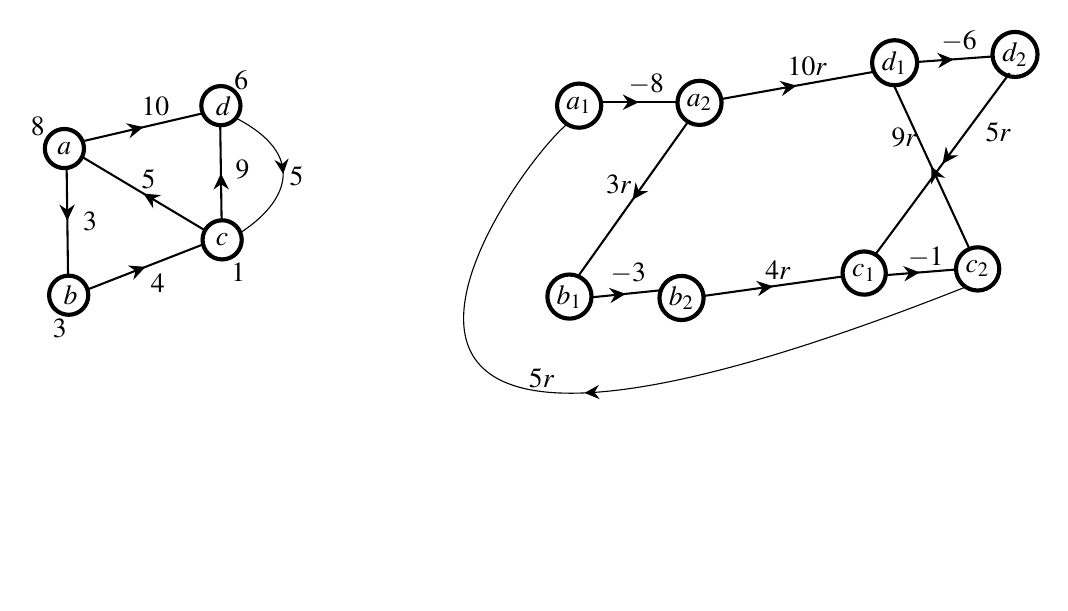
\begin{tikzpicture}[x=0.5pt,y=0.5pt,yscale=-1,xscale=1]
%uncomment if require: \path (0,288); %set diagram left start at 0, and has height of 288

%Straight Lines [id:da15240395104529547] 
\draw [color={rgb, 255:red, 0; green, 0; blue, 0 }  ,draw opacity=1 ][line width=0.75]    (51,102) -- (138,154) ;
\draw [shift={(94.5,128)}, rotate = 30.87] [fill={rgb, 255:red, 0; green, 0; blue, 0 }  ,fill opacity=1 ][line width=0.08]  [draw opacity=0] (11.61,-5.58) -- (0,0) -- (11.61,5.58) -- (7.71,0) -- cycle    ;
%Straight Lines [id:da35482909520855144] 
\draw [color={rgb, 255:red, 0; green, 0; blue, 0 }  ,draw opacity=1 ][line width=0.75]    (137,165) -- (55,197) ;
\draw [shift={(96,181)}, rotate = 158.68] [fill={rgb, 255:red, 0; green, 0; blue, 0 }  ,fill opacity=1 ][line width=0.08]  [draw opacity=0] (11.61,-5.58) -- (0,0) -- (11.61,5.58) -- (7.71,0) -- cycle    ;
%Straight Lines [id:da9934926023449607] 
\draw [color={rgb, 255:red, 0; green, 0; blue, 0 }  ,draw opacity=1 ][line width=0.75]    (39,109) -- (40,186) ;
\draw [shift={(39.5,147.5)}, rotate = 269.26] [fill={rgb, 255:red, 0; green, 0; blue, 0 }  ,fill opacity=1 ][line width=0.08]  [draw opacity=0] (11.61,-5.58) -- (0,0) -- (11.61,5.58) -- (7.71,0) -- cycle    ;
%Straight Lines [id:da7563500509285274] 
\draw [color={rgb, 255:red, 0; green, 0; blue, 0 }  ,draw opacity=1 ][line width=0.75]    (150,79) -- (151,148) ;
\draw [shift={(150.5,113.5)}, rotate = 89.17] [fill={rgb, 255:red, 0; green, 0; blue, 0 }  ,fill opacity=1 ][line width=0.08]  [draw opacity=0] (11.61,-5.58) -- (0,0) -- (11.61,5.58) -- (7.71,0) -- cycle    ;
%Straight Lines [id:da920349957299462] 
\draw [color={rgb, 255:red, 0; green, 0; blue, 0 }  ,draw opacity=1 ][line width=0.75]    (137.5,70) -- (51.5,90) ;
\draw [shift={(94.5,80)}, rotate = 166.91] [fill={rgb, 255:red, 0; green, 0; blue, 0 }  ,fill opacity=1 ][line width=0.08]  [draw opacity=0] (11.61,-5.58) -- (0,0) -- (11.61,5.58) -- (7.71,0) -- cycle    ;
%Curve Lines [id:da976908539012527] 
\draw    (160.5,73) .. controls (213.5,100) and (199.5,134) .. (163.5,157) ;
\draw [shift={(195.5,113.84)}, rotate = 263.76] [fill={rgb, 255:red, 0; green, 0; blue, 0 }  ][line width=0.08]  [draw opacity=0] (10.72,-5.15) -- (0,0) -- (10.72,5.15) -- (7.12,0) -- cycle    ;
%Straight Lines [id:da7434532828630788] 
\draw [color={rgb, 255:red, 0; green, 0; blue, 0 }  ,draw opacity=1 ][line width=0.75]    (479.5,62) -- (425.5,62) ;
\draw [shift={(452.5,62)}, rotate = 180] [fill={rgb, 255:red, 0; green, 0; blue, 0 }  ,fill opacity=1 ][line width=0.08]  [draw opacity=0] (11.61,-5.58) -- (0,0) -- (11.61,5.58) -- (7.71,0) -- cycle    ;
%Straight Lines [id:da3779476173807036] 
\draw [color={rgb, 255:red, 0; green, 0; blue, 0 }  ,draw opacity=1 ][line width=0.75]    (467.5,198) -- (418.5,203) ;
\draw [shift={(443,200.5)}, rotate = 174.17] [fill={rgb, 255:red, 0; green, 0; blue, 0 }  ,fill opacity=1 ][line width=0.08]  [draw opacity=0] (11.61,-5.58) -- (0,0) -- (11.61,5.58) -- (7.71,0) -- cycle    ;
%Straight Lines [id:da6132299382946279] 
\draw [color={rgb, 255:red, 0; green, 0; blue, 0 }  ,draw opacity=1 ][line width=0.75]    (680.5,183) -- (630.5,187) ;
\draw [shift={(655.5,185)}, rotate = 175.43] [fill={rgb, 255:red, 0; green, 0; blue, 0 }  ,fill opacity=1 ][line width=0.08]  [draw opacity=0] (11.61,-5.58) -- (0,0) -- (11.61,5.58) -- (7.71,0) -- cycle    ;
%Straight Lines [id:da8250679630157668] 
\draw [color={rgb, 255:red, 0; green, 0; blue, 0 }  ,draw opacity=1 ][line width=0.75]    (707.5,29) -- (652.5,33) ;
\draw [shift={(680,31)}, rotate = 175.84] [fill={rgb, 255:red, 0; green, 0; blue, 0 }  ,fill opacity=1 ][line width=0.08]  [draw opacity=0] (11.61,-5.58) -- (0,0) -- (11.61,5.58) -- (7.71,0) -- cycle    ;
%Straight Lines [id:da07369024589592021] 
\draw [color={rgb, 255:red, 0; green, 0; blue, 0 }  ,draw opacity=1 ][line width=0.75]    (408.5,188) -- (487.5,77) ;
\draw [shift={(448,132.5)}, rotate = 305.44] [fill={rgb, 255:red, 0; green, 0; blue, 0 }  ,fill opacity=1 ][line width=0.08]  [draw opacity=0] (11.61,-5.58) -- (0,0) -- (11.61,5.58) -- (7.71,0) -- cycle    ;
%Straight Lines [id:da320585315348929] 
\draw [color={rgb, 255:red, 0; green, 0; blue, 0 }  ,draw opacity=1 ][line width=0.75]    (599.5,188) -- (499.5,202) ;
\draw [shift={(549.5,195)}, rotate = 172.03] [fill={rgb, 255:red, 0; green, 0; blue, 0 }  ,fill opacity=1 ][line width=0.08]  [draw opacity=0] (11.61,-5.58) -- (0,0) -- (11.61,5.58) -- (7.71,0) -- cycle    ;
%Curve Lines [id:da28058077156757066] 
\draw    (687.5,196) .. controls (149.5,409) and (359.5,112) .. (400.5,78) ;
\draw [shift={(413.28,272.08)}, rotate = 356.86] [fill={rgb, 255:red, 0; green, 0; blue, 0 }  ][line width=0.08]  [draw opacity=0] (10.72,-5.15) -- (0,0) -- (10.72,5.15) -- (7.12,0) -- cycle    ;
%Straight Lines [id:da43509653737521126] 
\draw [color={rgb, 255:red, 0; green, 0; blue, 0 }  ,draw opacity=1 ][line width=0.75]    (636.5,49) -- (691.5,168) ;
\draw [shift={(664,108.5)}, rotate = 65.19] [fill={rgb, 255:red, 0; green, 0; blue, 0 }  ,fill opacity=1 ][line width=0.08]  [draw opacity=0] (11.61,-5.58) -- (0,0) -- (11.61,5.58) -- (7.71,0) -- cycle    ;
%Straight Lines [id:da6639766439417539] 
\draw [color={rgb, 255:red, 0; green, 0; blue, 0 }  ,draw opacity=1 ][line width=0.75]    (623.5,172) -- (720.5,41) ;
\draw [shift={(672,106.5)}, rotate = 306.52] [fill={rgb, 255:red, 0; green, 0; blue, 0 }  ,fill opacity=1 ][line width=0.08]  [draw opacity=0] (11.61,-5.58) -- (0,0) -- (11.61,5.58) -- (7.71,0) -- cycle    ;
%Straight Lines [id:da10266580678651627] 
\draw [color={rgb, 255:red, 0; green, 0; blue, 0 }  ,draw opacity=1 ][line width=0.75]    (622.5,40) -- (510.5,60) ;
\draw [shift={(566.5,50)}, rotate = 169.88] [fill={rgb, 255:red, 0; green, 0; blue, 0 }  ,fill opacity=1 ][line width=0.08]  [draw opacity=0] (11.61,-5.58) -- (0,0) -- (11.61,5.58) -- (7.71,0) -- cycle    ;

% Text Node
\draw (91.24,108.53) node [anchor=north west][inner sep=0.75pt]   [align=left] {$\displaystyle 5$};
% Text Node
\draw  [line width=1.5]   (37.38, 95.47) circle [x radius= 14.15, y radius= 14.15]   ;
\draw (37.38,95.47) node   [align=left] {$\displaystyle a$};
% Text Node
\draw  [line width=1.5]   (40.48, 201.47) circle [x radius= 14.15, y radius= 14.15]   ;
\draw (34.98,201.47) node [anchor=west] [inner sep=0.75pt]   [align=left] {$\displaystyle b$};
% Text Node
\draw  [line width=1.5]   (151.38, 161.47) circle [x radius= 14.15, y radius= 14.15]   ;
\draw (151.38,161.47) node   [align=left] {$\displaystyle c$};
% Text Node
\draw (98,184) node [anchor=north west][inner sep=0.75pt]   [align=left] {$\displaystyle 4$};
% Text Node
\draw (49,139.47) node [anchor=north west][inner sep=0.75pt]   [align=left] {$\displaystyle 3$};
% Text Node
\draw  [line width=1.5]   (150.48, 64.47) circle [x radius= 14.15, y radius= 14.15]   ;
\draw (144.98,64.47) node [anchor=west] [inner sep=0.75pt]   [align=left] {$\displaystyle d$};
% Text Node
\draw (159.24,101.53) node [anchor=north west][inner sep=0.75pt]   [align=left] {$\displaystyle 9$};
% Text Node
\draw (91.24,56.53) node [anchor=north west][inner sep=0.75pt]   [align=left] {$\displaystyle 10$};
% Text Node
\draw (11.24,70.53) node [anchor=north west][inner sep=0.75pt]   [align=left] {$\displaystyle 8$};
% Text Node
\draw (27.24,216.53) node [anchor=north west][inner sep=0.75pt]   [align=left] {$\displaystyle 3$};
% Text Node
\draw (156.24,176.53) node [anchor=north west][inner sep=0.75pt]   [align=left] {$\displaystyle 1$};
% Text Node
\draw (158.24,37.53) node [anchor=north west][inner sep=0.75pt]   [align=left] {$\displaystyle 6$};
% Text Node
\draw (198.24,106.53) node [anchor=north west][inner sep=0.75pt]   [align=left] {$\displaystyle 5$};
% Text Node
\draw  [line width=1.5]   (409.38, 64.47) circle [x radius= 15.95, y radius= 15.95]   ;
\draw (409.38,64.47) node   [align=left] {$\displaystyle a_{1}$};
% Text Node
\draw  [line width=1.5]   (496.38, 62.47) circle [x radius= 15.95, y radius= 15.95]   ;
\draw (496.38,62.47) node   [align=left] {$\displaystyle a_{2}$};
% Text Node
\draw  [line width=1.5]   (402.38, 202.47) circle [x radius= 15.95, y radius= 15.95]   ;
\draw (402.38,202.47) node   [align=left] {$\displaystyle b_{1}$};
% Text Node
\draw  [line width=1.5]   (483.38, 203.47) circle [x radius= 15.95, y radius= 15.95]   ;
\draw (483.38,203.47) node   [align=left] {$\displaystyle b_{2}$};
% Text Node
\draw  [line width=1.5]   (615.38, 185.47) circle [x radius= 15.62, y radius= 15.62]   ;
\draw (615.38,185.47) node   [align=left] {$\displaystyle c_{1}$};
% Text Node
\draw  [line width=1.5]   (697.38, 182.47) circle [x radius= 15.62, y radius= 15.62]   ;
\draw (697.38,182.47) node   [align=left] {$\displaystyle c_{2}$};
% Text Node
\draw  [line width=1.5]   (637.38, 33.47) circle [x radius= 16.28, y radius= 16.28]   ;
\draw (637.38,33.47) node   [align=left] {$\displaystyle d_{1}$};
% Text Node
\draw  [line width=1.5]   (724.38, 27.47) circle [x radius= 16.28, y radius= 16.28]   ;
\draw (724.38,27.47) node   [align=left] {$\displaystyle d_{2}$};
% Text Node
\draw (443.24,39.53) node [anchor=north west][inner sep=0.75pt]   [align=left] {$\displaystyle -8$};
% Text Node
\draw (430.24,176.53) node [anchor=north west][inner sep=0.75pt]   [align=left] {$\displaystyle -3$};
% Text Node
\draw (645.24,164.53) node [anchor=north west][inner sep=0.75pt]   [align=left] {$\displaystyle -1$};
% Text Node
\draw (669.24,8.53) node [anchor=north west][inner sep=0.75pt]   [align=left] {$\displaystyle -6$};
% Text Node
\draw (558.24,27.53) node [anchor=north west][inner sep=0.75pt]   [align=left] {$\displaystyle 10r$};
% Text Node
\draw (371.24,252.53) node [anchor=north west][inner sep=0.75pt]   [align=left] {$\displaystyle 5r$};
% Text Node
\draw (427,112.47) node [anchor=north west][inner sep=0.75pt]   [align=left] {$\displaystyle 3r$};
% Text Node
\draw (542,175) node [anchor=north west][inner sep=0.75pt]   [align=left] {$\displaystyle 4r$};
% Text Node
\draw (633.24,78.53) node [anchor=north west][inner sep=0.75pt]   [align=left] {$\displaystyle 9r$};
% Text Node
\draw (701.24,74.53) node [anchor=north west][inner sep=0.75pt]   [align=left] {$\displaystyle 5r$};


\end{tikzpicture}

}
\vspace{-2.6cm}
\caption{Constructing $G_1$ from $G$ and $r$.}
\label{fig:cycle}
\end{figure}


Hence, we can keep writing above reasoning:
\begin{eqnarray*}
& & r < r^* \\
& \Longleftrightarrow & \exists \textrm{ cycle } C \textrm{ in $G$ s.t.\ } \textstyle \sum_{e\in C} r\cdot c(e) + \sum_{v\in C} (-p(v)) < 0 \\
& \Longleftrightarrow & \exists \textrm{ cycle } C_1 \textrm{ in $G_1$ s.t.\ the length of $C_1$ is smaller than 0 } \\
& \Longleftrightarrow & \textrm{ $G_1$ contains negative cycle } \\
\end{eqnarray*}

We therefore successfully transformed the problem of deciding if $r < r^*$ into a problem of deciding if $G_1$ contains negative cycle,
which we know how to solve.
The pseudo-code is given below.

\begin{minipage}{0.8\textwidth}
	\aaA {5}{Algorithm decide-lower-bound~($G = (V, E)$, $r$)}\xxx
	\aab {build $G_1 = (V_1, E_1)$;}\xxx
	\aab {call an algorithm to decide if $G_1$ contains negative cycle;}\xxx
	\aab {if $G_1$ contains negative cycle: return true~(i.e., $r < r^*$);}\xxx
	\aab {else: return false~(i.e., $r \ge r^*$);}\xxx
	\aaa {end algorithm;}\xxx
\end{minipage}

The running time of above algorithm is dominated by the procedure of deciding negativ cycles, which is $O(|V_1|\cdot |E_1|)$.
Notice that $|V_1| = 2|V|$ and $|E_1| = |V| + |E|$. Hence, the running time of above algorithm is $O(|V|^2 + |V| \cdot |E|)$.


\subsection*{Initial Bounds}

We now find an initial bounds $r_1$ and $r_2$ for $r^*$.
We can use a trivial lower bound, i.e., $r_1 = 0$.
What is a possible upper bound of $r^*$?
Notice that $r(C)$ is the ratio of the sum of vertex-profits and the sum of edge-costs,
and the number of vertices and the number of edges in a cycle are the same.
Hence, we have an upper bound: $r_2 = \max_{v\in V} p(v) / \max_{e\in E} c(e)$.
A better upper bound can be obtained by realizing that in any cycle edge $e = (u,v)$ is always followed by vertex $v$.
Hence, we have a better bound: $r_2 = \max_{e = (u,v) \in E} p(v) / c(e)$.

\subsection*{Running Time Analysis}

To see the running time, assume $t$ is the number of iterations in the binary search.
We have $(r_2 - r_1) / 2^t = \epsilon$. Hence we have $t = \log (r_2 / \epsilon)$.
The overall running time is therefore $O(\log (r_2 / \epsilon) (|V|^2 + |V||E|))$.
Notice that this running time is a function of $\epsilon$, as expected.
Notice too, that this running time involves numeric value, i.e., $r_2 / \epsilon$.
The \emph{input-size} of any numeric value $x$ is $\log x$.
Therefore $\log(r_2 / \epsilon)$ is linear in the input-size of $r_2/\epsilon$.
Hence, the entire algorithm runs in polynomial-time.

To comapre, consider the linear-search algorithm given below.

\begin{minipage}{0.8\textwidth}
	\aaA {5}{Algorithm linear-search~($G = (V, E)$, $a$, $b$)}\xxx
	\aab {init $r = 0$;}\xxx
	\aab {let $z$ = decide-lower-bound~($G$, $r$);}\xxx
	\aab {if $z$ = true: $r = r + \epsilon$;}\xxx
	\aab {else: return $(r - \epsilon, r]$;}\xxx
	\aaa {end algorithm;}\xxx
\end{minipage}

This algorithm is correct, but it may call decide-lower-bound $r_2 / \epsilon$ times.
So its overall running time is $O(r_2 / \epsilon (|V|^2 + |V||E|))$.
This is \emph{not} a polynomial-time algorithm,
as $r_2 / \epsilon$ is exponential in its input-size, which is $\log(r_2/\epsilon)$.

In conclusion, binary-search is essential to achieve an efficient algorithm for this problem.

\subsection*{Finding A Negative Cycle}

We know how to extend DP or BF algorithms to decide the existence of a negative cycle.
If it exists, how to actually find one?
Again, we can use the shortest-path graph, i.e., $G' = (V, \{(prev[v], v) \mid v\in V\})$ constructed
from the $prev$ array. Note, this $prev$ array is associated with the row-$|V|$ in the DP algorithm,
or associated with the $|V|$-th iterations of the BF algorithm.
We can prove that, if $G$ contains negative cycle, then this graph $G'$ must contain cycle,
and any cycle in $G'$ must be a negative cycle of $G$. See an example below.

\begin{figure}[h]
\centering{

\tikzset{every picture/.style={line width=0.75pt}} %set default line width to 0.75pt        

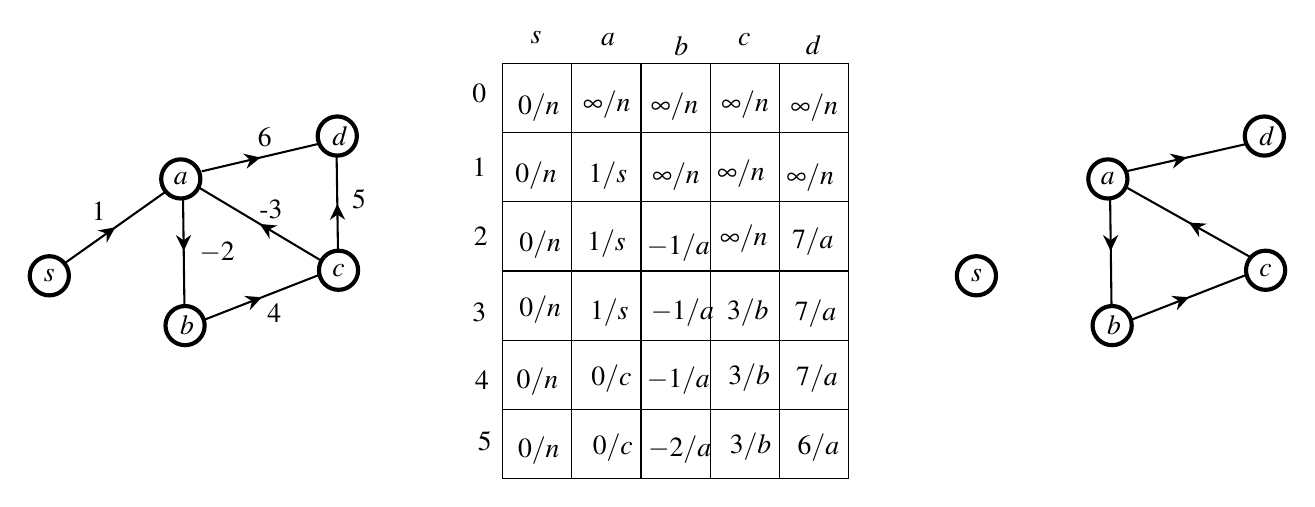
\begin{tikzpicture}[x=0.5pt,y=0.5pt,yscale=-1,xscale=1]
%uncomment if require: \path (0,384); %set diagram left start at 0, and has height of 384

%Shape: Grid [id:dp11668880045661734] 
\draw  [draw opacity=0] (366,45) -- (616,45) -- (616,345) -- (366,345) -- cycle ; \draw   (416,45) -- (416,345)(466,45) -- (466,345)(516,45) -- (516,345)(566,45) -- (566,345) ; \draw   (366,95) -- (616,95)(366,145) -- (616,145)(366,195) -- (616,195)(366,245) -- (616,245)(366,295) -- (616,295) ; \draw   (366,45) -- (616,45) -- (616,345) -- (366,345) -- cycle ;
%Straight Lines [id:da34498379019209924] 
\draw [color={rgb, 255:red, 0; green, 0; blue, 0 }  ,draw opacity=1 ][line width=0.75]    (50,189) -- (122,138) ;
\draw [shift={(86,163.5)}, rotate = 504.69] [fill={rgb, 255:red, 0; green, 0; blue, 0 }  ,fill opacity=1 ][line width=0.08]  [draw opacity=0] (11.61,-5.58) -- (0,0) -- (11.61,5.58) -- (7.71,0) -- cycle    ;
%Straight Lines [id:da15240395104529547] 
\draw [color={rgb, 255:red, 0; green, 0; blue, 0 }  ,draw opacity=1 ][line width=0.75]    (147,135) -- (234,187) ;
\draw [shift={(190.5,161)}, rotate = 30.87] [fill={rgb, 255:red, 0; green, 0; blue, 0 }  ,fill opacity=1 ][line width=0.08]  [draw opacity=0] (11.61,-5.58) -- (0,0) -- (11.61,5.58) -- (7.71,0) -- cycle    ;
%Straight Lines [id:da35482909520855144] 
\draw [color={rgb, 255:red, 0; green, 0; blue, 0 }  ,draw opacity=1 ][line width=0.75]    (233,198) -- (151,230) ;
\draw [shift={(192,214)}, rotate = 158.68] [fill={rgb, 255:red, 0; green, 0; blue, 0 }  ,fill opacity=1 ][line width=0.08]  [draw opacity=0] (11.61,-5.58) -- (0,0) -- (11.61,5.58) -- (7.71,0) -- cycle    ;
%Straight Lines [id:da9934926023449607] 
\draw [color={rgb, 255:red, 0; green, 0; blue, 0 }  ,draw opacity=1 ][line width=0.75]    (135,142) -- (136,219) ;
\draw [shift={(135.5,180.5)}, rotate = 269.26] [fill={rgb, 255:red, 0; green, 0; blue, 0 }  ,fill opacity=1 ][line width=0.08]  [draw opacity=0] (11.61,-5.58) -- (0,0) -- (11.61,5.58) -- (7.71,0) -- cycle    ;
%Straight Lines [id:da7563500509285274] 
\draw [color={rgb, 255:red, 0; green, 0; blue, 0 }  ,draw opacity=1 ][line width=0.75]    (246,112) -- (247,181) ;
\draw [shift={(246.5,146.5)}, rotate = 89.17] [fill={rgb, 255:red, 0; green, 0; blue, 0 }  ,fill opacity=1 ][line width=0.08]  [draw opacity=0] (11.61,-5.58) -- (0,0) -- (11.61,5.58) -- (7.71,0) -- cycle    ;
%Straight Lines [id:da1926158580753592] 
\draw [color={rgb, 255:red, 0; green, 0; blue, 0 }  ,draw opacity=1 ][line width=0.75]    (906.5,185) -- (817.5,135) ;
\draw [shift={(862,160)}, rotate = 389.33000000000004] [fill={rgb, 255:red, 0; green, 0; blue, 0 }  ,fill opacity=1 ][line width=0.08]  [draw opacity=0] (11.61,-5.58) -- (0,0) -- (11.61,5.58) -- (7.71,0) -- cycle    ;
%Straight Lines [id:da5417396008779365] 
\draw [color={rgb, 255:red, 0; green, 0; blue, 0 }  ,draw opacity=1 ][line width=0.75]    (903,198) -- (821,230) ;
\draw [shift={(862,214)}, rotate = 158.68] [fill={rgb, 255:red, 0; green, 0; blue, 0 }  ,fill opacity=1 ][line width=0.08]  [draw opacity=0] (11.61,-5.58) -- (0,0) -- (11.61,5.58) -- (7.71,0) -- cycle    ;
%Straight Lines [id:da8796336265405228] 
\draw [color={rgb, 255:red, 0; green, 0; blue, 0 }  ,draw opacity=1 ][line width=0.75]    (805,142) -- (806,219) ;
\draw [shift={(805.5,180.5)}, rotate = 269.26] [fill={rgb, 255:red, 0; green, 0; blue, 0 }  ,fill opacity=1 ][line width=0.08]  [draw opacity=0] (11.61,-5.58) -- (0,0) -- (11.61,5.58) -- (7.71,0) -- cycle    ;
%Straight Lines [id:da08409930095041618] 
\draw [color={rgb, 255:red, 0; green, 0; blue, 0 }  ,draw opacity=1 ][line width=0.75]    (904.5,103) -- (816.5,123) ;
\draw [shift={(860.5,113)}, rotate = 167.2] [fill={rgb, 255:red, 0; green, 0; blue, 0 }  ,fill opacity=1 ][line width=0.08]  [draw opacity=0] (11.61,-5.58) -- (0,0) -- (11.61,5.58) -- (7.71,0) -- cycle    ;
%Straight Lines [id:da920349957299462] 
\draw [color={rgb, 255:red, 0; green, 0; blue, 0 }  ,draw opacity=1 ][line width=0.75]    (233.5,103) -- (148.5,123) ;
\draw [shift={(191,113)}, rotate = 166.76] [fill={rgb, 255:red, 0; green, 0; blue, 0 }  ,fill opacity=1 ][line width=0.08]  [draw opacity=0] (11.61,-5.58) -- (0,0) -- (11.61,5.58) -- (7.71,0) -- cycle    ;

% Text Node
\draw (375.24,65.06) node [anchor=north west][inner sep=0.75pt]   [align=left] {$\displaystyle 0/n$};
% Text Node
\draw (342.24,111.56) node [anchor=north west][inner sep=0.75pt]   [align=left] {$\displaystyle 1$};
% Text Node
\draw (343.24,161.06) node [anchor=north west][inner sep=0.75pt]   [align=left] {$\displaystyle 2$};
% Text Node
\draw (384.24,19.56) node [anchor=north west][inner sep=0.75pt]   [align=left] {$\displaystyle s$};
% Text Node
\draw (435.24,21.56) node [anchor=north west][inner sep=0.75pt]   [align=left] {$\displaystyle a$};
% Text Node
\draw (488.24,23.56) node [anchor=north west][inner sep=0.75pt]   [align=left] {$\displaystyle b$};
% Text Node
\draw (534.24,21.56) node [anchor=north west][inner sep=0.75pt]   [align=left] {$\displaystyle c$};
% Text Node
\draw (422.24,63.06) node [anchor=north west][inner sep=0.75pt]   [align=left] {$\displaystyle \infty /n$};
% Text Node
\draw (342.24,58.06) node [anchor=north west][inner sep=0.75pt]   [align=left] {$\displaystyle 0$};
% Text Node
\draw (342.24,216.06) node [anchor=north west][inner sep=0.75pt]   [align=left] {$\displaystyle 3$};
% Text Node
\draw (188.24,141.53) node [anchor=north west][inner sep=0.75pt]   [align=left] {\mbox{-}$\displaystyle 3$};
% Text Node
\draw  [line width=1.5]   (38.38, 198.47) circle [x radius= 14.15, y radius= 14.15]   ;
\draw (38.38,198.47) node   [align=left] {$\displaystyle s$};
% Text Node
\draw  [line width=1.5]   (133.38, 128.47) circle [x radius= 14.15, y radius= 14.15]   ;
\draw (133.38,128.47) node   [align=left] {$\displaystyle a$};
% Text Node
\draw  [line width=1.5]   (136.48, 234.47) circle [x radius= 14.15, y radius= 14.15]   ;
\draw (130.98,234.47) node [anchor=west] [inner sep=0.75pt]   [align=left] {$\displaystyle b$};
% Text Node
\draw  [line width=1.5]   (247.38, 194.47) circle [x radius= 14.15, y radius= 14.15]   ;
\draw (247.38,194.47) node   [align=left] {$\displaystyle c$};
% Text Node
\draw (67.24,143.53) node [anchor=north west][inner sep=0.75pt]   [align=left] {$\displaystyle 1$};
% Text Node
\draw (194,217) node [anchor=north west][inner sep=0.75pt]   [align=left] {$\displaystyle 4$};
% Text Node
\draw (145,172.47) node [anchor=north west][inner sep=0.75pt]   [align=left] {$\displaystyle -2$};
% Text Node
\draw (471.24,64.06) node [anchor=north west][inner sep=0.75pt]   [align=left] {$\displaystyle \infty /n$};
% Text Node
\draw (522.24,63.06) node [anchor=north west][inner sep=0.75pt]   [align=left] {$\displaystyle \infty /n$};
% Text Node
\draw (519.24,113.06) node [anchor=north west][inner sep=0.75pt]   [align=left] {$\displaystyle \infty /n$};
% Text Node
\draw (373.24,114.06) node [anchor=north west][inner sep=0.75pt]   [align=left] {$\displaystyle 0/n$};
% Text Node
\draw (376.24,164.06) node [anchor=north west][inner sep=0.75pt]   [align=left] {$\displaystyle 0/n$};
% Text Node
\draw (376.24,211.06) node [anchor=north west][inner sep=0.75pt]   [align=left] {$\displaystyle 0/n$};
% Text Node
\draw (426.24,114.06) node [anchor=north west][inner sep=0.75pt]   [align=left] {$\displaystyle 1/s$};
% Text Node
\draw (472.24,115.06) node [anchor=north west][inner sep=0.75pt]   [align=left] {$\displaystyle \infty /n$};
% Text Node
\draw (521.24,160.06) node [anchor=north west][inner sep=0.75pt]   [align=left] {$\displaystyle \infty /n$};
% Text Node
\draw (425.24,163.06) node [anchor=north west][inner sep=0.75pt]   [align=left] {$\displaystyle 1/s$};
% Text Node
\draw (468.24,166.06) node [anchor=north west][inner sep=0.75pt]   [align=left] {$\displaystyle -1/a$};
% Text Node
\draw (344.24,265.06) node [anchor=north west][inner sep=0.75pt]   [align=left] {$\displaystyle 4$};
% Text Node
\draw (583.24,22.56) node [anchor=north west][inner sep=0.75pt]   [align=left] {$\displaystyle d$};
% Text Node
\draw  [line width=1.5]   (246.48, 97.47) circle [x radius= 14.15, y radius= 14.15]   ;
\draw (240.98,97.47) node [anchor=west] [inner sep=0.75pt]   [align=left] {$\displaystyle d$};
% Text Node
\draw (255.24,134.53) node [anchor=north west][inner sep=0.75pt]   [align=left] {$\displaystyle 5$};
% Text Node
\draw (572.24,65.06) node [anchor=north west][inner sep=0.75pt]   [align=left] {$\displaystyle \infty /n$};
% Text Node
\draw (569.24,116.06) node [anchor=north west][inner sep=0.75pt]   [align=left] {$\displaystyle \infty /n$};
% Text Node
\draw (573.24,162.06) node [anchor=north west][inner sep=0.75pt]   [align=left] {$\displaystyle 7/a$};
% Text Node
\draw (575.24,214.06) node [anchor=north west][inner sep=0.75pt]   [align=left] {$\displaystyle 7/a$};
% Text Node
\draw (374.24,263.06) node [anchor=north west][inner sep=0.75pt]   [align=left] {$\displaystyle 0/n$};
% Text Node
\draw (427.24,213.06) node [anchor=north west][inner sep=0.75pt]   [align=left] {$\displaystyle 1/s$};
% Text Node
\draw (471.24,213.06) node [anchor=north west][inner sep=0.75pt]   [align=left] {$\displaystyle -1/a$};
% Text Node
\draw (468.24,262.06) node [anchor=north west][inner sep=0.75pt]   [align=left] {$\displaystyle -1/a$};
% Text Node
\draw (526.24,213.06) node [anchor=north west][inner sep=0.75pt]   [align=left] {$\displaystyle 3/b$};
% Text Node
\draw (527.24,260.06) node [anchor=north west][inner sep=0.75pt]   [align=left] {$\displaystyle 3/b$};
% Text Node
\draw (576.24,261.06) node [anchor=north west][inner sep=0.75pt]   [align=left] {$\displaystyle 7/a$};
% Text Node
\draw (428.24,261.06) node [anchor=north west][inner sep=0.75pt]  [color={rgb, 255:red, 208; green, 2; blue, 27 }  ,opacity=1 ] [align=left] {$\displaystyle \textcolor[rgb]{0,0,0}{0/c}$};
% Text Node
\draw  [line width=1.5]   (708.38, 198.47) circle [x radius= 14.15, y radius= 14.15]   ;
\draw (708.38,198.47) node   [align=left] {$\displaystyle s$};
% Text Node
\draw  [line width=1.5]   (803.38, 128.47) circle [x radius= 14.15, y radius= 14.15]   ;
\draw (803.38,128.47) node   [align=left] {$\displaystyle a$};
% Text Node
\draw  [line width=1.5]   (806.48, 234.47) circle [x radius= 14.15, y radius= 14.15]   ;
\draw (800.98,234.47) node [anchor=west] [inner sep=0.75pt]   [align=left] {$\displaystyle b$};
% Text Node
\draw  [line width=1.5]   (917.38, 194.47) circle [x radius= 14.15, y radius= 14.15]   ;
\draw (917.38,194.47) node   [align=left] {$\displaystyle c$};
% Text Node
\draw  [line width=1.5]   (916.48, 97.47) circle [x radius= 14.15, y radius= 14.15]   ;
\draw (910.98,97.47) node [anchor=west] [inner sep=0.75pt]   [align=left] {$\displaystyle d$};
% Text Node
\draw (187.24,89.53) node [anchor=north west][inner sep=0.75pt]   [align=left] {$\displaystyle 6$};
% Text Node
\draw (375.24,313.06) node [anchor=north west][inner sep=0.75pt]   [align=left] {$\displaystyle 0/n$};
% Text Node
\draw (469.24,312.06) node [anchor=north west][inner sep=0.75pt]   [align=left] {$\displaystyle -2/a$};
% Text Node
\draw (528.24,310.06) node [anchor=north west][inner sep=0.75pt]   [align=left] {$\displaystyle 3/b$};
% Text Node
\draw (577.24,311.06) node [anchor=north west][inner sep=0.75pt]   [align=left] {$\displaystyle 6/a$};
% Text Node
\draw (429.24,311.06) node [anchor=north west][inner sep=0.75pt]  [color={rgb, 255:red, 208; green, 2; blue, 27 }  ,opacity=1 ] [align=left] {$\displaystyle \textcolor[rgb]{0,0,0}{0/c}$};
% Text Node
\draw (346.24,309.06) node [anchor=north west][inner sep=0.75pt]   [align=left] {$\displaystyle 5$};


\end{tikzpicture}

}
\caption{Find a negative cycle using $prev$ array.}
\label{fig:dpbf}
\end{figure}


\end{document}
